
% Prepared for Cargèse, September 2016. Four lectures of 50 minutes each. 


\documentclass[12pt, a4paper]{article}

\raggedbottom

\RequirePackage[l2tabu, orthodox]{nag}

\usepackage[top=20mm,bottom=20mm,left=25mm,right=25mm]{geometry}

\usepackage{showkeys}

\usepackage{amsfonts, amsmath}

\usepackage{pgf}
\usepackage{tikz}

\usepackage{multirow}

\usepackage{pgf}
\usepackage{tikz}

\usepackage{amsthm}

\makeatletter
% \def\@endtheorem{\endtrivlist\@endpefalse }% OLD
\def\@endtheorem{\endtrivlist}% NEW
\makeatother

\newtheoremstyle{break}{9pt}{9pt}{\itshape}{}{\bfseries}{}{\newline}{}
\theoremstyle{break}    
\newtheorem{exo}{Exercise}[section]
\newtheorem{hyp}[exo]{Axiom}
\newtheorem{res}[exo]{Result}
\newtheorem{defn}[exo]{Definition}

\usepackage[colorlinks=true,linktoc=all,linkcolor=black,citecolor=red,urlcolor=blue]{hyperref}

\title{\bfseries Minimal lectures on two-dimensional \\ conformal field theory}

\author{Sylvain Ribault \vspace{2mm}
\\
{\normalsize CEA Saclay, Institut de Physique Th\'eorique}
 \\
 {\footnotesize \ttfamily sylvain.ribault@ipht.fr }
}

\begin{document}


\maketitle


\begin{abstract}
We provide a brief but self-contained review of conformal field theory on the Riemann sphere. We first introduce general axioms such as local conformal invariance, and derive Ward identities and BPZ equations. We then define minimal models and  Liouville theory by specific axioms on their spectrums and degenerate fields. We solve these theories by computing 
three- and four-point functions, and discuss their existence and uniqueness. 
\end{abstract}

\vspace{5mm}

 \noindent\textit{Lectures given at the Carg\`ese school on ``Quantum integrable systems, conformal field theories and stochastic processes'' in September 2016, under the title ``Conformal bootstrap approach to Liouville theory''.}



\clearpage

\tableofcontents

\hypersetup{linkcolor=blue}

\numberwithin{equation}{section}
\setcounter{section}{-1}

\section{Introduction}

Since the time of Euclid, mathematical objects are defined by axioms. 
Axiomatic definitions focus on the basic features of the defined objects, thereby avoiding alternative constructions that may be less fundamental.
For example, in conformal field theory, the axiomatic approach (also called the conformal bootstrap approach) makes functional integrals unnecessary.
We will define Liouville theory and minimal models by a sequence of axioms, starting with local conformal symmetry. 
Our axioms are necessary conditions. 
Their mutual consistency, in other words the existence of Liouville theory and minimal models, will be tested but not proved.

In the first three sections, most axioms are common to all two-dimensional conformal field theories.
These axioms specify in particular how the Virasoro symmetry algebra acts on fields, and the existence and properties of the operator product expansion. 
Next, we introduce additional axioms that single out either Liouville theory, or minimal models.
In particular, these axioms determine the three-point functions. 
Finally we check that these uniquely defined theories do exist, by studying their four-point functions.

This text was written with brevity as the main concern, so as to be the basis for about four hours' worth of lectures. For more details along these lines, see the review article \cite{rib14}. For a wider and more advanced review in a similar spirit, see Teschner's recent text \cite{tes17}. 
The Bible of rational conformal field theory is of course the epic textbook \cite{fms97}. And Cardy's lecture notes \cite{car08} provide an introduction to the statistical physics applications of conformal field theory.


\section{The Virasoro algebra and its representations}

\subsection{Algebra}

By definition, conformal transformations are transformations that preserve angles. 
In two dimensions with a complex coordinate $z$, any holomorphic transformation preserves angles.
Infinitesimal conformal transformations are holomorphic functions close to the identity function, 
\begin{align}
 z \mapsto z + \epsilon z^{n+1}\qquad (n\in\mathbb{Z}\ , \ \epsilon\ll 1) \ .
\end{align}
These transformations act on functions of $z$ via the differential operators 
\begin{align}
 \ell_n = -z^{n+1}\frac{\partial}{\partial z}\ ,
\end{align}
and these operators generate the Witt algebra, with commutation relations
\begin{align}
 [\ell_n,\ell_m ] = (n-m)\ell_{m+n}\ .
\end{align}
The generators $(\ell_{-1},\ell_0,\ell_1)$ generate an $s\ell_2$ subalgebra, called the algebra of infinitesimal global conformal transformations.  The corresponding Lie group is the group of conformal transformations of 
the Riemann sphere $\mathbb{C}\cup \{\infty\}$,
\begin{align}
 z \mapsto \frac{az+b}{cz+d}\ .
\end{align}

\begin{exo}[Global conformal group of the sphere]
 ~\label{exo:sphere}
Show that the global conformal group of the sphere is $PSL_2(\mathbb{C})$, and includes translations, rotations, and dilatations. 
\end{exo}

In a quantum theory, symmetry transformations act projectively on states. 
Projective representations of an algebra are equivalent to representations of a centrally extended algebra. 
This is why we always look for central extensions of symmetry algebras.

\begin{defn}[Virasoro algebra]
 ~\label{def:vir}
 The central extension of the Witt algebra is called the Virasoro algebra. It has the generators $(L_n)_{n\in\mathbb{Z}}$ and $\mathbf 1$, and the commutation relations
 \begin{align}
  [\mathbf 1, L_n] = 0 \quad , \quad [L_n,L_m] = (n-m)L_{n+m} +\frac{c}{12}(n-1)n(n+1)\delta_{n+m,0}\mathbf 1 \ ,
  \label{eq:vir}
 \end{align}
 where the number $c$ is called the central charge. (The notation $c\mathbf 1$ stands for a central generator that always has the same eigenvalue $c$ in a given conformal field theory.)
\end{defn}

\begin{exo}[Uniqueness of the Virasoro algebra]
 ~\label{exo:vir}
 Show that the Virasoro algebra is the unique central extension of the Witt algebra.
\end{exo}


\subsection{Representations}

The spectrum, i.e. the space of states, must be a representation of the Virasoro algebra. Let us now make assumptions on what type of representation it can be.

\begin{hyp}[Representations that can appear in the spectrum]
 ~\label{hyp:rep}
 The spectrum is a direct sum of irreducible representations. In the spectrum, $L_0$ is diagonalizable, and the real part of its eigenvalues is bounded from below.
\end{hyp}
Why this special role for $L_0$? Because we want to interpret it as the energy operator. Since the corresponding Witt algebra generator $\ell_0$ generates dilatations, considering it as the energy operator amounts to consider the radial coordinate as the time. We however do not assume that $L_0$ eigenvalues are real or that the spectrum is a Hilbert space, as this would restrict the central charge to be real. The $L_0$ eigenvalue of an $L_0$ eigenvector is called its conformal dimension.

Let us consider an irreducible representation that is allowed by our axiom. There must be an $L_0$ eigenvector $|v\rangle$ with the smallest eigenvalue $\Delta$. Then $L_n|v\rangle$ is also an $L_0$ eigenvector,
\begin{align}
 L_0 L_n|v\rangle = L_nL_0|v\rangle + [L_0, L_n] |v\rangle  = (\Delta-n)L_n|v\rangle \ .
\end{align}
If $n>0$ we must have $L_n|v\rangle =0$, and $|v\rangle $ is called a primary state.

\begin{defn}[Primary and descendent states, level, Verma module]
 ~\label{def:prim}
 A primary state with conformal dimension $\Delta$ is a state $|v\rangle$ such that 
 \begin{align}
  L_0 |v\rangle = \Delta |v\rangle \quad , \quad L_{n>0} |v\rangle = 0\ .
 \end{align}
The Verma module $\mathcal V_\Delta$ is the representation whose basis is 
 $
 \left\{ \prod_{i=1}^k L_{-n_i} |v\rangle\right\}_{ 0<n_1\leq \dots \leq n_k}
 $.
The level of the state $\prod_{i=1}^k L_{-n_i} |v\rangle $ is $N=\sum_{i=1}^k n_i\geq 0$. A state of level $N\geq 1$ is called a descendent state.
\end{defn}
Let us plot a basis of primary and descendent states up to the level $3$:
\begin{align}
 \begin{tikzpicture}[scale = .25, baseline=(current  bounding  box.center)]
  \draw[-latex, very thick] (20, 0) -- (20, -21) node [right] {$N$};
  \foreach \x in {0, ..., 3}
  {
  \draw [dotted] (-20, {-6*\x}) -- (20, {-6*\x}) node [right] {${\x}$};
  }
  \node[fill = white] at (0, 0) (0) {$|v\rangle$};
  \node[fill = white] at (-4,-6) (1) {$L_{-1}|v\rangle$};
  \node[fill = white] at (-8, -12) (11) {$L_{-1}^2|v\rangle$};
  \node[fill = white] at (-12, -18) (111) {$L_{-1}^3|v\rangle$};
  \node[fill = white] at (0,-12) (2) {$L_{-2}|v\rangle$};
  \node[fill = white] at (0,-18) (12) {$L_{-1}L_{-2}|v\rangle$};
  \node[fill = white] at (8,-18) (3) {$L_{-3}|v\rangle$};
  \draw[-latex] (0) -- (1);
  \draw[-latex] (1) -- (11);
  \draw[-latex] (11) -- (111);
  \draw[-latex] (0) -- (2);
  \draw[-latex] (0) -- (3);
  \draw[-latex] (2) -- (12);
 \end{tikzpicture}
\end{align}
We need not include the state $L_{-2}L_{-1}|v\rangle$, due to $L_{-2}L_{-1} = L_{-1}L_{-2} - L_{-3}$.

Are Verma module irreducible representations? i.e. do they have nontrivial subrepresentations? In any subrepresentation of a Verma module, $L_0$ is again diagonalizable and bounded from below, so there must be a primary state $|\chi\rangle$. If the subrepresentation differs from the Verma module, that primary state must differ from $|v\rangle$, and therefore be a descendent of $|v\rangle$.

\subsection{Null vectors and degenerate representations}\label{sec:nv}

\begin{defn}[Null vectors]
 ~\label{def:nv}
 A descendent state that is also primary is called a null vector or singular vector.
\end{defn}
In the Verma module $\mathcal V_\Delta$, let us look for null vectors at the level $N=1$. For $n\geq 1$ we have 
\begin{align}
L_n L_{-1}|v\rangle = [L_n, L_{-1}] |v\rangle = (n+1) L_{n-1}|v\rangle = 
\left\{\begin{array}{ll} 0 &  \quad \text{if } n\geq 2 \\ 2\Delta |v\rangle & \quad \text{if } n = 1 \end{array}\right. 
\end{align}
So $L_{-1}|v\rangle$ is a null vector if and only if $\Delta=0$, and the Verma module $\mathcal V_0$ is reducible.
Let us now look for null vectors at the level $N=2$. Let $|\chi\rangle = (L_{-1}^2 + a L_{-2})|v\rangle$, then $L_{n\geq 3} |\chi \rangle =0$. 

\begin{exo}
 ~\label{exo:level2}
 Compute  $L_1|\chi\rangle$ and $L_2|\chi\rangle$, and find 
 \begin{align}
  L_1 |\chi\rangle = \left((4\Delta+2) + 3a\right) L_{-1}|v\rangle
  \quad , \quad L_2 |\chi\rangle= \left(6\Delta + (4\Delta +\tfrac12 c)a\right) |v\rangle\ .
 \end{align}
 Requiring that $L_1|\chi\rangle$ and $L_2|\chi\rangle$ vanish, find the coefficient $a$, and show that
 \begin{align}
 \Delta = \frac{1}{16}\left( 5-c\pm\sqrt{(c-1)(c-25)} \right) \ .
 \label{eq:dpm}
\end{align}
\end{exo}
In order to simplify this formula, let us introduce other notations for $c$ and $\Delta$. We define
\begin{align}
 \text{the background charge } Q \ , & \quad c = 1+6Q^2\ , \quad \text{up to } Q \to -Q\ ,
 \\
 \text{the coupling constant } b \ , & \quad Q = b+\frac{1}{b} \ , \quad \text{up to } b\to \pm b^{\pm 1}\ ,
 \\
 \text{the momentum } \alpha\  , &\quad \Delta = \alpha(Q-\alpha)\ , \quad \text{up to reflections } \alpha \to Q-\alpha\ .
\label{eq:refm}
 \end{align}
The condition \eqref{eq:dpm} for the existence of a level two null vector becomes 
\begin{align}
 \alpha = -\frac12 b^{\pm 1}\ .
\end{align}
To summarize, null vectors at levels $1$ and $2$ occur for particular values of $\Delta$. The null vectors at levels $N\leq 2$ can be written as $L_{\langle r,s\rangle}|v\rangle$ where $r,s$ are strictly positive integers such that $rs=N$,
\begin{align}
\renewcommand{\arraystretch}{1.3}
\begin{array}{|c|c|c|c|c|}
\hline 
N & \langle r,s\rangle & \Delta_{\langle r,s\rangle} & \alpha_{\langle r,s\rangle} & L_{\langle r,s\rangle} 
\\
\hline\hline
1 & \langle 1,1\rangle & 0 & 0 & L_{-1}
\\
\hline
\multirow{2}{*}{2} & 
\langle 2,1\rangle & -\frac12 -\frac{3}{4} b^2 & -\frac{b}{2} & L_{-1}^2 + b^2 L_{-2}
\\
\cline{2-5}
& \langle 1,2\rangle & -\frac12 - \frac{3}{4b^2} &  -\frac{1}{2b} & L_{-1}^2 + b^{-2} L_{-2} 
\\
\hline
\end{array}
\label{lot}
\end{align}
The pattern goes on at higher levels \cite{fms97}: null vectors occur at level $N$ for finitely many dimensions $\Delta_{\langle r,s\rangle}$, with
\begin{align}
  \alpha_{\langle r,s\rangle} = \frac{Q}{2} - \frac12(rb+sb^{-1})\ .
  \label{eq:ars}
 \end{align}
 (See Exercise \ref{exo:hdr} for a derivation.)
If $\Delta\notin\{\Delta_{\langle r,s\rangle}\}_{r,s\in\mathbb{N}^*}$, then $\mathcal V_\Delta$ is irreducible. If $\Delta = \Delta_{\langle r,s\rangle}$, then $\mathcal V_\Delta$ contains a nontrivial submodule, generated by the null vector and its descendent states. For generic values of the central charge $c$, this submodule is the Verma module $\mathcal V_{\Delta_{\langle r,s\rangle}+rs}$.

\begin{defn}[Degenerate representation]
 ~\label{def:deg}
The coset of the reducible Verma module $\mathcal V_{\Delta_{\langle r,s\rangle}}$, by its Verma submodule $\mathcal V_{\Delta_{\langle r,s\rangle}+rs}$, is an irreducible module $\mathcal{R}_{\langle r,s\rangle}$, that is called a degenerate representation:
\begin{align}
 \mathcal{R}_{\langle r,s\rangle} = \frac{\mathcal V_{\Delta_{\langle r,s\rangle}}}{\mathcal V_{\Delta_{\langle r,s\rangle}+rs}}
\end{align}
In this representation, the null vector vanishes,
\begin{align}
 L_{\langle r,s\rangle}|v\rangle = 0\ .
\end{align}
\end{defn}
The vanishing of null vectors will be crucial for solving Liouville theory and minimal models.


\section{Conformal field theory}\label{sec:cft}

Now that we understand the algebraic structure of conformal symmetry in two dimensions, let us study how the Virasoro algebra acts on objects that live on the Riemann sphere -- the fields of conformal field theory. (Technically, fields are sections of vector bundles over the sphere.)

\subsection{Fields}

\begin{hyp}[State-field correspondence]
 ~\label{hyp:sfc}
For any state $|w\rangle$ in the spectrum, there is an associated field $V_{|w\rangle}(z)$. The map $|w\rangle \mapsto V_{|w\rangle}(z)$ is linear. We define the action of the Virasoro algebra on such fields as 
\begin{align}
 L_n V_{|w\rangle}(z) =  L_n^{(z)} V_{|w\rangle}(z) = V_{L_n|w\rangle}(z)\ .
\end{align}
\end{hyp}

\begin{defn}[Primary field, descendent field, degenerate field]
~\label{def:pfdf}
Let $|v\rangle$ be the primary state of the Verma module $\mathcal V_\Delta$.
We define the primary field $V_\Delta(z)=V_{|v\rangle}(z)$. This field obeys
\begin{align}
 L_{n\geq 0} V_\Delta(z) = 0 \quad , \quad L_0 V_\Delta(z) = \Delta V_\Delta(z)\ .
\end{align}
Similarly, descendent fields correspond to descendent states. And the degenerate field $V_{\langle r,s\rangle}(z)$ corresponds to the primary state of the degenerate representation $\mathcal{R}_{\langle r,s\rangle}$, and therefore obeys 
\begin{align}
 L_{\langle r, s\rangle} V_{\langle r,s\rangle}(z) = 0\qquad \text{-- for example, \ } L_{-1}V_{\langle 1,1\rangle}(z) = 0\ .
\end{align}
\end{defn}

Now let us specify how fields depend on $z$. 

\begin{hyp}[Dependence of fields on $z$]
 ~\label{hyp:geom}
 For any field $V(z)$, we have 
 \begin{align}
  \frac{\partial}{\partial z} V(z) = L_{-1} V(z)  \ .
  \label{pvlv}
 \end{align}
\end{hyp}
Moreover, in this Section \ref{sec:cft} we tacitly assume that all our fields are locally holomorphic i.e. $\frac{\partial}{\partial \bar z} V(z) = 0$. The dependence on $\bar z$ will be reintroduced and studied in Section \ref{sec:sv}.

Let us derive consequences of this axiom, starting with the $z$-dependence of the action $L_n^{(z)}$ of Virasoro generators on fields. On the one hand,
\begin{align}
 \frac{\partial}{\partial z} \left( L_n^{(z)} V(z) \right) = \left(\frac{\partial}{\partial z} L_n^{(z)}\right) V(z) + L_n^{(z)} \frac{\partial}{\partial z} V(z)\ .
\end{align}
On the other hand, using our axiom, we find 
\begin{align}
 \frac{\partial}{\partial z} \left( L_n^{(z)} V(z) \right) = L_{-1}^{(z)} L_n^{(z)} V(z) = -(n+1)L_{n-1}^{(z)} V(z) + L_n^{(z)} L_{-1}^{(z)} V(z)\ .
\end{align}
This implies 
\begin{align}
 \frac{\partial}{\partial z} L_n^{(z)} = -(n+1)L_{n-1}^{(z)}\ ,\qquad (\forall n\in\mathbb{Z})\ .
\end{align}
These infinitely many equations can be encoded into one functional equation,
\begin{align}
 \frac{\partial}{\partial z} \sum_{n\in\mathbb{Z}} \frac{L_n^{(z)}}{(y-z)^{n+2}} = 0\ .
\end{align}

\begin{defn}[Energy-momentum tensor]
 ~\label{def:em}
 The energy-momentum tensor is a field, that we define by the formal Laurent series
 \begin{align}
  T(y) = \sum_{n\in\mathbb{Z}} \frac{L_n^{(z)}}{(y-z)^{n+2}} \ .
 \end{align}
In other words, for any field $V(z)$, we have 
\begin{align}
 T(y)V(z) = \sum_{n\in\mathbb{Z}} \frac{L_n V(z)}{(y-z)^{n+2}}\quad , \quad L_n V(z) = \frac{1}{2\pi i} \oint_{z}dy\ (y-z)^{n+1} T(y)V(z)\ .
 \label{eq:lvtv}
\end{align}
\end{defn}
In the case of a primary field $V_\Delta(z)$, using eq. \eqref{pvlv} and writing regular terms as $O(1)$, this definition reduces to
\begin{align}
 T(y)V_\Delta(z) = \frac{\Delta}{(y-z)^2} V_\Delta(z) + \frac{1}{y-z} \frac{\partial}{\partial z} V_\Delta(z) + O(1)\ . 
 \label{eq:tvd}
\end{align}
This is our first example of an operator product expansion.

The energy-momentum tensor $T(y)$ is locally holomorphic as a function of $y$, and acquires poles in the presence of other fields. Since we are on the Riemann sphere, it must also be holomorphic at $y=\infty$. 

\begin{hyp}[Behaviour of $T(y)$ at infinity]
~\label{hyp:ti}
 \begin{align}
 T(y) \underset{y\to\infty} = O\left(\frac{1}{y^4}\right)\ .
 \label{eq:tinf}
\end{align}
\end{hyp}
To motivate this axiom, let us do some dimensional analysis. If $z$ has dimension $-1$, then according to eq. \eqref{pvlv} $L_{-1}$ has dimension $1$, and $T(y)$ has dimension $2$. The dimensionless quantity that should be holomorphic at infinity is therefore the differential $T(y)dy^2$. At infinity a holomorphic coordinate is $\frac{1}{y}$ and a holomorphic differential is $d(\frac{1}{y}) = -\frac{dy}{y^2}$, so our axiom amounts to $T(y)dy^2= O(\frac{dy^2}{y^4})$ being holomorphic.


\subsection{Correlation functions and Ward identities}

\begin{defn}[Correlation function]
~\label{def:cor}
 To $N$ fields $V_1(z_1), \dots ,V_N(z_N)$ with $i\neq j\Rightarrow z_i\neq z_j$, we associate a number called their correlation function or $N$-point function, and denoted as 
 \begin{align}
  \Big< V_1(z_1) \cdots V_N(z_N) \Big>\ .
 \end{align}
For example, $\left< \prod_{i=1}^N V_{\Delta_i}(z_i) \right>$ is a function of $\{z_i\}, \{\Delta_i\}$ and $c$.
Correlation functions depend linearly on fields, and in particular $\frac{\partial}{\partial z_1} \left< V_1(z_1) \cdots V_N(z_N) \right> = \left< \frac{\partial}{\partial z_1}V_1(z_1) \cdots V_N(z_N) \right>$.
\end{defn}

\begin{hyp}[Commutativity of fields]
 ~\label{hyp:ass}
 Correlation functions do not depend on the order of the fields,
 \begin{align}
  V_1(z_1) V_2(z_2) = V_2(z_2)V_1(z_1)\ .
 \end{align}
\end{hyp}

Let us work out the consequences of conformal symmetry for correlation functions.
In order to study an $N$-point function $Z$ of primary fields, we introduce an auxiliary $(N+1)$-point function $Z(y)$ where we insert the energy-momentum tensor,
\begin{align}
 Z = \left< \prod_{i=1}^N V_{\Delta_i}(z_i) \right> \quad , \quad Z(y) = \left< T(y) \prod_{i=1}^N V_{\Delta_i}(z_i) \right> \ .
\end{align}
$Z(y)$ is a meromorphic function of $y$, with poles at $y=z_i$, whose residues are given by eq. \eqref{eq:tvd} (using the commutativity of fields).
Moreover $T(y)$, and therefore also $Z(y)$, vanish in the limit $y\to \infty$. So $Z(y)$ is completely determined by its poles and residues,
\begin{align}
 Z(y) = \sum_{i=1}^N \left(\frac{\Delta_i}{(y-z_i)^2} +\frac{1}{y-z_i}\frac{\partial}{\partial z_i}\right) Z\ .
 \label{eq:zy}
\end{align}
But $T(y)$ is not just bounded for $y\to \infty$, it behaves as $O(\frac{1}{y^4})$.
So the coefficients of $y^{-1}, y^{-2}, y^{-3}$ in the large $y$ expansion of $Z(y)$ must vanish, 
\begin{align}
 \sum_{i=1}^N \partial_{z_i} Z = \sum_{i=1}^N \left(z_i \partial_{z_i} + \Delta_i\right) Z = \sum_{i=1}^N \left(z_i^2 \partial_{z_i} + 2\Delta_iz_i\right) Z = 0\ .
 \label{eq:gward}
\end{align}
These three equations are called global Ward identities. They determine how $Z$ behaves under global conformal transformations of the Riemann sphere,
\begin{align}
 \left< \prod_{i=1}^N  V_{\Delta_i}\left(\frac{az_i+b}{cz_i+d}\right) \right>
 = \prod_{i=1}^N (cz_i +d)^{2\Delta_i} \left< \prod_{i=1}^N V_{\Delta_i}(z_i) \right>\ .
 \label{eq:zgc}
\end{align}
Let us solve the global Ward identities in the cases of one, two, three and four-point functions. For a one-point function, we have 
\begin{align}
\partial_z \Big< V_\Delta(z)\Big> = 0 \quad , \quad \Delta \Big< V_\Delta(z)\Big> = 0\ .
\end{align}
So one-point functions are constant, and non-vanishing only if $\Delta=0$. Similarly, two-point functions must obey
\begin{align}
 \Big< V_{\Delta_1}(z_1)V_{\Delta_2}(z_2) \Big> \propto (z_1-z_2)^{-2\Delta_1} \quad , \quad (\Delta_1-\Delta_2)\Big< V_{\Delta_1}(z_1)V_{\Delta_2}(z_2) \Big>  = 0\ .
 \label{eq:2pt}
\end{align}
So a two-point function can be non-vanishing only if the two fields have the same dimension.
For three-point functions, there are as many equations \eqref{eq:gward} as unknowns $z_1,z_2,z_3$, and therefore a unique solution with no constraints on $\Delta_i$,
\begin{align}
 \left< \prod_{i=1}^3 V_{\Delta_i}(z_i) \right> \propto (z_1-z_2)^{\Delta_3-\Delta_1-\Delta_2} (z_1-z_3)^{\Delta_2-\Delta_1-\Delta_3} (z_2-z_3)^{\Delta_1-\Delta_2-\Delta_3}\ ,
 \label{eq:3pt}
\end{align}
with an unknown proportionality coefficient that does not depend on $z_i$.
For four-point functions, the general solution is
\begin{align}
 \left< \prod_{i=1}^4 V_{\Delta_i}(z_i) \right> = \left(\prod_{i<j}(z_i-z_j)^{\delta_{ij}}\right) G\left(\frac{(z_1-z_2)(z_3-z_4)}{(z_1-z_3)(z_2-z_4)}\right)\ ,
\end{align}
where $G$ is an arbitrary function, and $\delta_{ij}$ are such that $\sum_{j\neq i} \delta_{ij} = -2\Delta_i$, where $\delta_{ij}\underset{i>j}{=}\delta_{ji}$. The six numbers $\delta_{ij}$ with $i<j$ are subject to only four equations, leaving two undetermined combinations. Changing these combinations amounts to a redefinition $G(z)\to z^\lambda (1-z)^\mu G(z)$.

In other words, the three global Ward identities effectively reduces the four-point function to a function of one variable $G$ -- equivalently, we can set $z_2,z_3,z_4$ to fixed values, and recover the four-point function from its dependence on $z_1$ alone. 

\begin{exo}[Conformal symmetry of four-point functions]
~\label{exo:4pt}
 Let us define $V_\Delta(\infty) = \lim_{z\to\infty} z^{2\Delta}V_\Delta(z) $. Check that this is finite when inserted into a two- or three-point function. More generally, show that this is finite using the behaviour \eqref{eq:zgc} of correlation functions under $z\to -\frac{1}{z}$. 
 Show that there is a (unique) choice of $\delta_{ij}$ such that 
 \begin{align}
  G(z) = \Big< V_{\Delta_1}(z) V_{\Delta_2}(0)V_{\Delta_3}(\infty)V_{\Delta_4}(1) \Big>\ .
 \end{align}
\end{exo}

We have been studying global conformal invariance of correlation functions of primary fields, rather than more general fields. This was not only for making things simpler, but also because correlation functions of descendents can be deduced from correlation functions of primaries. For example,
\begin{align}
 \Big< L_{-2}V_{\Delta_1}(z_1) V_{\Delta_2}(z_2)\cdots \Big>
  = \frac{1}{2\pi i}\oint_{z_1} \frac{dy}{y-z_1} Z(y)
  =\sum_{i=2}^N\left(\frac{1}{z_1-z_i}\frac{\partial}{\partial z_i} +\frac{\Delta_i}{(z_i-z_1)^2}\right) Z\ ,
  \label{eq:ltv}
\end{align}
where we used first eq. \eqref{eq:lvtv} for $L_{-2}V_{\Delta_1}(z_1)$, and then eq. \eqref{eq:zy} for $Z(y)$.
This can be generalized to any correlation function of descendent fields. The resulting equations are called local Ward identities.


\subsection{Belavin--Polyakov--Zamolodchikov equations}

Local and global Ward identities are all we can deduce from conformal symmetry. But correlation functions that involve degenerate fields obey additional equations. 

For example, let us replace $V_{\Delta_1}(z_1)$ with the degenerate primary field $V_{\langle 1, 1 \rangle}(z_1)$
in our $N$-point function $Z$. Since $\frac{\partial}{\partial z_1} V_{\langle 1, 1 \rangle}(z_1) = L_{-1} V_{\langle 1, 1 \rangle}(z_1) =0$,
we obtain $\frac{\partial}{\partial z_1} Z =0$. 
In the case $N=3$, having $\Delta_1=\Delta_{\langle 1,1\rangle}=0$ in the three-point function \eqref{eq:3pt} leads to
\begin{align}
 \left< V_{\langle 1, 1 \rangle}(z_1) V_{\Delta_2}(z_2) V_{\Delta_3}(z_3) \right> \propto (z_1-z_2)^{\Delta_3-\Delta_2} (z_1-z_3)^{\Delta_2-\Delta_3} (z_2-z_3)^{-\Delta_2-\Delta_3}\ , 
\end{align}
and further imposing $z_1$-independence leads to 
\begin{align}
 \left< V_{\langle 1, 1 \rangle}(z_1) V_{\Delta_2}(z_2) V_{\Delta_3}(z_3) \right> \neq 0 \quad \Rightarrow \quad \Delta_2=\Delta_3\ .
\end{align}
This coincides with the condition \eqref{eq:2pt} that the two-point function $\left<V_{\Delta_2}(z_2)V_{\Delta_3}(z_3)\right>$ does not vanish. Actually, the field $V_{\langle 1,1\rangle}$ is an identity field, i.e. a field whose presence does not affect correlation functions. (See Exercise \ref{exo:id}.)

In the case of $V_{\langle 2, 1 \rangle}(z_1)$, we have  
\begin{align}
\left(L_{-1}^2 + b^2 L_{-2}\right) V_{\langle 2, 1 \rangle}(z_1)  = 0\qquad \text{so that} \qquad L_{-2}V_{\langle 2, 1 \rangle}(z_1) = -\frac{1}{b^2}\frac{\partial^2}{\partial z_1^2} V_{\langle 2, 1 \rangle}(z_1)\ .
\end{align}
Using the local Ward identity \eqref{eq:ltv},
this leads to the second-order Belavin--Polyakov--Zamolodchikov partial differential equation
\begin{align}
 \left( \frac{1}{b^2}\frac{\partial^2}{\partial z_1^2} + \sum_{i=2}^N\left(\frac{1}{z_1-z_i}\frac{\partial}{\partial z_i} +\frac{\Delta_i}{(z_1-z_i)^2}\right) \right)\left< V_{\langle 2, 1 \rangle}(z_1) \prod_{i=2}^N V_{\Delta_i}(z_i) \right>  = 0\ .
 \label{eq:bpz}
\end{align}
More generally, a correlation function with the degenerate field $V_{\langle r,s\rangle}$ obeys a partial differential equation of order $rs$. 

\begin{exo}[Second-order BPZ equation for a three-point function]
 ~\label{exo:bpz3pt}
 Show that 
\begin{align}
 \left< V_{\langle 2, 1 \rangle} V_{\Delta_2} V_{\Delta_3} \right> \neq 0 \quad \Rightarrow \quad 
 2(\Delta_2-\Delta_3)^2 +b^2(\Delta_2+\Delta_3) -2\Delta_{\langle 2, 1 \rangle}^2 -b^2\Delta_{\langle 2, 1 \rangle} = 0\ .
 \end{align}
 Up to reflections of momentums, show that this is equivalent to
 \begin{align}
 \alpha_2 = \alpha_3 \pm \frac{b}{2}\ .
 \label{eq:alpm}
\end{align}
\end{exo}

In the case of a four-point function, the BPZ equation amounts to a differential equation for the function of one variable $G(z)$, which therefore belongs to a finite-dimensional space of solutions.

\begin{exo}[BPZ second-order differential equation]
 ~\label{exo:bpz}
 Show that the second-order BPZ equation for $G(z)=\Big< V_{\langle 2, 1 \rangle}(z) V_{\Delta_1}(0)V_{\Delta_2}(\infty)V_{\Delta_3}(1) \Big>$ is
 \begin{align}
  \left\{ \frac{z(1-z)}{b^2}\frac{\partial^2}{\partial z^2} + (2z-1){\frac{\partial}{\partial z}} +\Delta_{\langle 2,1 \rangle} +\frac{\Delta_1}{z}-\Delta_2 + \frac{\Delta_3}{1-z}\right\} G(z)=0\ ,
\label{eq:ode}
 \end{align}
\end{exo}


\section{Conformal bootstrap}

We have seen how conformal symmetry leads to linear equations for correlation functions: Ward identities and BPZ equations. 
In order to fully determine correlation functions, we need additional, nonlinear equations, and therefore additional axioms: single-valuedness of correlation functions, and existence of operator product expansions. 
Using these axioms for studying conformal field theories is called the conformal bootstrap method. 

\subsection{Single-valuedness}\label{sec:sv}

\begin{hyp}[Single-valuedness]
 ~\label{hyp:sv}
 Correlation functions are single-valued functions of the positions, i.e. they have trivial monodromies.
\end{hyp}

Until now, our correlation functions are locally holomorphic functions of the type $z^\Delta$, as a result of solving holomorphic Ward identities. Single-valued correlation functions should be of the type $z^\Delta \bar z^\Delta$ instead. 
This suggests that we need anti-holomorphic Ward identities as well, and therefore a second copy of the Virasoro algebra.

\begin{hyp}[Left and right Virasoro algebras]
 ~\label{hyp:lr}
 We have two mutually commuting Virasoro symmetry algebras with the same central charge, called left-moving or holomorphic, and right-moving or anti-holomorphic. Their generators are written $L_n,\bar L_n$, with in particular
 \begin{align}
  \frac{\partial}{\partial z} V(z) = L_{-1}V(z)   \quad , \quad \frac{\partial}{\partial \bar z} V(z)= \bar L_{-1} V(z)   \ .
 \end{align}
 The generators of conformal transformations are the diagonal combinations $L_n+\bar L_n$.
\end{hyp}

Let us now consider left- and right-primary fields $V_{\Delta_i,\bar\Delta_i}(z_i)$. According to eq. \eqref{eq:3pt}, the three-point function is 
\begin{align}
 \left<\prod_{i=1}^3V_{\Delta_i,\bar\Delta_i}(z_i) \right> \propto (z_1-z_2)^{\Delta_3-\Delta_1-\Delta_2} (\bar z_1-\bar z_2)^{\bar\Delta_3-\bar\Delta_1-\bar\Delta_2} \times \cdots\ .
\end{align}
Single-valuedness as a function of $z_i$ constrains the spins $s_i=\Delta_i-\bar\Delta_i$, 
\begin{align}
 s_i+s_j-s_k \in \mathbb{Z}\ .
\end{align}
This implies in particular $2s_i\in\mathbb{Z}$. In other words, any primary field $V_{\Delta,\bar\Delta}(z)$ must obey
\begin{align}
 \Delta -\bar \Delta \in \frac12\mathbb{Z}\ .
\end{align} 
The simplest case is $\Delta=\bar\Delta$, which leads to the definition

\begin{defn}[Diagonal states, diagonal fields and diagonal spectrums]
 ~\label{def:diag}
 A primary state or field is called diagonal if it has the same left and right conformal dimensions. A spectrum is called diagonal if all primary states are diagonal.
\end{defn}
From now on we will use the notation $V_\Delta(z)$ for the diagonal field $V_{\Delta,\Delta}(z)$.

\subsection{Operator product expansion and crossing symmetry}

\begin{hyp}[Operator product expansion]
 ~\label{hyp:ope}
 Let $V_1(z_1)$ and $V_2(z_2)$ be two fields, and $|w_i\rangle$ be a basis of the spectrum.
 There exist coefficients $C^i_{12}(z_1,z_2)$ such that we have the operator product expansion (OPE) 
 \begin{align}
  V_1(z_1)V_2(z_2) = \sum_i C^i_{12}(z_1,z_2) V_{|w_i\rangle}(z_2)\ .
 \end{align}
 In a correlation functions,
 this sum converges for $z_1$ sufficiently close to $z_2$.
\end{hyp}
If the spectrum is made of diagonal primary states and their descendent states, the OPE of two primary fields is
\begin{align}
 V_{\Delta_1}(z_1) V_{\Delta_2}(z_2) 
 = \sum_{\Delta\in S} C_{\Delta_1,\Delta_2,\Delta} |z_1-z_2|^{2(\Delta-\Delta_1-\Delta_2)}
 \Big(V_{\Delta}(z_2) + O(z_1-z_2) \Big)\ ,
 \label{eq:ope}
\end{align}
where the subleading terms are contributions of descendents fields. 
In particular, the $z_1,z_2$-dependence of the coefficients is dictated by global conformal invariance eq. \eqref{eq:zgc}, leaving a $z_i$-independent unknown factor $C_{\Delta_1,\Delta_2,\Delta}$.
Then, as in correlation functions, contributions of descendents are deduced from contributions of primaries via local Ward identitites.

\begin{exo}[Computing the OPE of primary fields]
~\label{exo:ope}
 Compute the first subleading term in the OPE \eqref{eq:ope}, and find
 \begin{align}
  O(z_1-z_2) = \frac{\Delta+\Delta_1-\Delta_2}{2\Delta} \Big( (z_1-z_2)L_{-1}+(\bar z_1-\bar z_2)\bar L_{-1}\Big) V_{\Delta}(z_2) + O((z_1-z_2)^2)\ .
 \end{align}
\end{exo}

\begin{exo}[$V_{\langle 1,1\rangle}$ as an identity field]
~\label{exo:id}
Using $\frac{\partial}{\partial z_1} V_{\langle 1,1\rangle}(z_1)=0$, show that the OPE of $V_{\langle 1,1\rangle}$ with another primary field is of the form 
\begin{align}
 V_{\langle 1,1\rangle}(z_1)V_\Delta(z_2) = C_\Delta V_\Delta(z_2)\ ,
\end{align}
where the subleading terms vanish. Inserting this OPE in a correlation function, show that the constant $C_\Delta$ actually does not depend on $\Delta$. Deduce that, up to a factor $C=C_\Delta$, the field $V_{\langle 1,1\rangle}$ is an identity field.
\end{exo}


Inserting the OPE in a three-point function of primary fields, we find 
\begin{align}
 \left<\prod_{i=1}^3 V_{\Delta_i}(z_i) \right> & = \sum_{\Delta\in S}C_{\Delta_1,\Delta_2,\Delta} |z_1-z_2|^{2(\Delta-\Delta_1-\Delta_2)}
 \Big(\left< V_{\Delta}(z_2) V_{\Delta_3}(z_3) \right> +O(z_1-z_2)\Big) \ ,
 \\
& =  C_{\Delta_1,\Delta_2,\Delta_3} |z_1-z_2|^{2(\Delta_3-\Delta_1-\Delta_2)} \Big( |z_2-z_3|^{-4\Delta_3} + O(z_1-z_2)\Big)\ ,
\end{align}
assuming the two-point function is normalized as $\left< V_{\Delta}(z_1)V_{\Delta}(z_2) \right> = |z_1-z_2|^{-4\Delta}$.
Therefore $C_{\Delta_1,\Delta_2,\Delta_3}$ coincides with the undertermined constant prefactor of the three-point function \eqref{eq:3pt}. This factor is called the three-point structure constant, and we have
\begin{align}
 \left<\prod_{i=1}^3 V_{\Delta_i}(z_i) \right> = C_{\Delta_1,\Delta_2,\Delta_3} |z_1-z_2|^{2(\Delta_3-\Delta_1-\Delta_2)} |z_1-z_3|^{2(\Delta_2-\Delta_1-\Delta_3)} |z_2-z_3|^{2(\Delta_1-\Delta_2-\Delta_3)}\ .
\end{align}
Let us now insert the OPE in a four-point function of primary fields:
\begin{align}
 \Big<V_{\Delta_1}(z)V_{\Delta_2}(0)V_{\Delta_3}(\infty)V_{\Delta_4}(1)\Big>
 &= \sum_{\Delta\in S} C_{\Delta_1,\Delta_2,\Delta} |z|^{2(\Delta-\Delta_1-\Delta_2)}
 \nonumber
\\ & \qquad \qquad \times 
 \left(\Big< V_\Delta(0)V_{\Delta_3}(\infty)V_{\Delta_4}(1)\Big> + O(z)\right) \ ,
 \\
 &=  \sum_{\Delta\in S} C_{\Delta_1,\Delta_2,\Delta} C_{\Delta,\Delta_3,\Delta_4}
|z|^{2(\Delta-\Delta_1-\Delta_2)} \Big(1 +O(z) \Big)\ .
\end{align}
The contributions of descendents factorize into those of left-moving descendents, generated by the operators $L_{n<0}$, and right-moving descendents, generated by $\bar L_{n<0}$. So the last factor has a holomorphic factorization such that 
\begin{align}
\Big<V_{\Delta_1}(z)V_{\Delta_2}(0)V_{\Delta_3}(\infty)V_{\Delta_4}(1)\Big>
 =\sum_{\Delta\in S} C_{\Delta_1,\Delta_2,\Delta} C_{\Delta,\Delta_3,\Delta_4}  \mathcal{F}^{(s)}_\Delta(z) \mathcal{F}^{(s)}_\Delta(\bar z)\ .
 \label{sdec}
\end{align}

\begin{defn}[Conformal block]
 ~\label{def:block}
 The four-point conformal block on the sphere,
 \begin{align}
  \mathcal{F}^{(s)}_\Delta(z) = z^{\Delta-\Delta_1-\Delta_2}\Big( 1 + O(z) \Big)\ ,
  \label{eq:gsd}
 \end{align}
is the normalized contribution of the Verma module $\mathcal V_\Delta$ to a four-point function, obtained by summing over left-moving descendents. Its dependence on $c,\Delta_1,\Delta_2,\Delta_3,\Delta_4$ are kept implicit. The label $(s)$ stands for for $s$-channel, we will soon see what this means.
\end{defn}
Conformal blocks are in principle known, as they are universal functions, entirely determined by conformal symmetry. This is analogous to characters of representations, also known as zero-point conformal blocks on the torus.

\begin{exo}[Computing conformal blocks]
 ~\label{exo:block}
 Compute the conformal block $ \mathcal{F}^{(s)}_\Delta(z)$ up to the order $O(z)$, and find
 \begin{align}
  \mathcal{F}^{(s)}_\Delta(z) = z^{\Delta-\Delta_1-\Delta_2}\left( 1 + \frac{(\Delta+\Delta_1-\Delta_2)(\Delta+\Delta_4-\Delta_3)}{2\Delta}z + O(z^2) \right)\ .
 \end{align}
 Discuss the pole at $\Delta=0$, and its disappearance for certain values of $\Delta_i$.
\end{exo}

Our axiom \ref{hyp:ass} on the commutativity of fields implies that the OPE is associative, and that we can use the OPE of any two fields in a four-point function. In particular, using the OPE of the first and fourth fields, we obtain 
\begin{align}
 \Big<V_{\Delta_1}(z)V_{\Delta_2}(0)V_{\Delta_3}(\infty)V_{\Delta_4}(1)\Big>
 =\sum_{\Delta\in S} C_{\Delta,\Delta_1,\Delta_4} C_{\Delta_2,\Delta_3,\Delta}   \mathcal{F}^{(t)}_\Delta(z) \mathcal{F}^{(t)}_\Delta(\bar z)\ ,
 \label{tdec}
\end{align}
where $\mathcal{F}^{(t)}_\Delta(z) = (z-1)^{\Delta-\Delta_1-\Delta_4}\Big(1+O(z-1)\Big)$ is a $t$-channel conformal block.
The equality of our two decompositions \eqref{sdec} and \eqref{tdec} of the four-point function is called crossing symmetry, schematically 
\begin{align}
 \sum_{\Delta_s\in S} C_{12s} C_{s34} 
 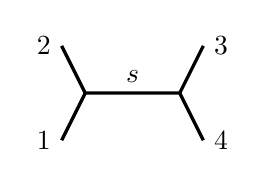
\begin{tikzpicture}[baseline=(current  bounding  box.center), very thick, scale = .3]
\draw (-1,2) node [left] {$2$} -- (0,0) -- node [above] {$s$} (4,0) -- (5,2) node [right] {$3$};
\draw (-1,-2) node [left] {$1$} -- (0,0);
\draw (4,0) -- (5,-2) node [right] {$4$};
\end{tikzpicture} 
= \sum_{\Delta_t\in S} C_{23t}C_{t41} 
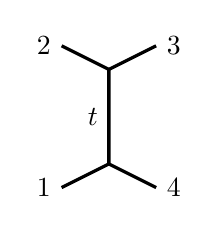
\begin{tikzpicture}[baseline=(current  bounding  box.center), very thick, scale = .3]
 \draw (-2,3) node [left] {$2$} -- (0,2) -- node [left] {$t$} (0,-2) -- (-2, -3) node [left] {$1$};
\draw (0,2) -- (2,3) node [right] {$3$};
\draw (0,-2) -- (2, -3) node [right] {$4$};
\end{tikzpicture}
\ .
\label{csd}
\end{align}
This equation holds if the sums on both sides converge, that is if $z$ is sufficiently close to both $0$ and $1$,
\begin{align}
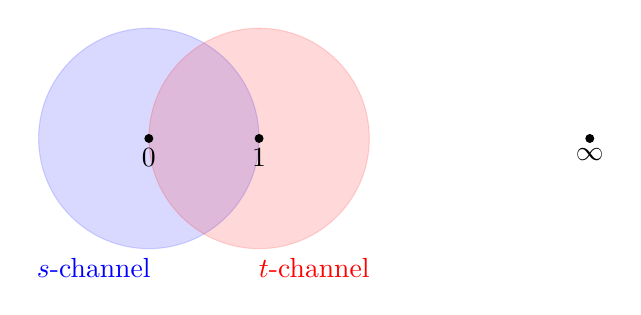
\begin{tikzpicture}[scale = 1.4, baseline=(current  bounding  box.center)]
 \filldraw[blue, opacity = .15] (0, 0) circle [radius = 1];
 \filldraw[red, opacity = .15] (1, 0) circle [radius = 1];
 \filldraw (0, 0) circle [radius = 1pt] node [below] {$0$};
 \filldraw (1, 0) circle [radius = 1pt] node [below] {$1$};
 \filldraw (4, 0) circle [radius = 1pt] node [below] {$\infty$};
 \node[below, blue] at (-.5, -1) {$s$-channel};
 \node[below, red] at (1.5, -1) {$t$-channel};
\end{tikzpicture}
\end{align}
Given the spectrum $S$, crossing symmetry is a system of quadratic equations for the structure constant $C_{\Delta_1,\Delta_2,\Delta_3}$. Requiring that this system has solutions is a strong constraint on the spectrum. 


\subsection{Degenerate fields and the fusion product}

Crossing symmetry equations are powerful, but typically involve infinite sums, which makes them difficult to solve.
However, if at least one field is degenerate, then the four-point function belongs to the finite-dimensional space of solutions of a BPZ equation, and is therefore a combination of finitely many conformal blocks. 
For example,
$\Big< V_{\langle 2, 1 \rangle}(z) V_{\Delta_1}(0)V_{\Delta_2}(\infty)V_{\Delta_3}(1) \Big>$ is a combination of only two holomorphic $s$-channel conformal blocks.
These blocks are a particular basis of solutions of the BPZ equation \eqref{eq:ode}, characterized by their asymptotic behaviour near $z=0$ \eqref{eq:gsd}, 
\begin{align}
\mathcal{F}^{(s)}_{\alpha_1-\frac{b}{2}}(z) = z^{b\alpha_1} (1-z)^{b\alpha_3} F(A,B,C,z)\quad , \quad 
 \mathcal{F}^{(s)}_{\alpha_1+\frac{b}{2}}(z) = \left. \mathcal{F}^{(s)}_{\alpha_1-\frac{b}{2}}(z) \right|_{\alpha_1\to Q-\alpha_1} \ ,
\label{gpm}
\end{align}
where $F(A,B,C,z)$ is the hypergeometric function with parameters
\begin{align}
\renewcommand{\arraystretch}{1.3}
\left\{\begin{array}{l}   A = \frac12 + b(\alpha_1+\alpha_3-Q) + b(\alpha_2-\tfrac{Q}{2}) \ , \\
      B = \frac12 + b(\alpha_1+\alpha_3-Q) - b(\alpha_2-\tfrac{Q}{2}) \ , \\
      C = 1 + b(2\alpha_1-Q) \ .
\end{array}\right. 
\label{abc}
\end{align}
Similarly, the two relevant $t$-channel blocks are 
\begin{align}
 \mathcal{F}^{(t)}_{\alpha_3-\frac{b}{2}}(z) &= z^{b\alpha_1} (1-z)^{b\alpha_3} F(A,B,A+B-C+1,1-z)\ ,
 \nonumber \\
 \mathcal{F}^{(t)}_{\alpha_3+\frac{b}{2}}(z) &= \left. \mathcal{F}^{(t)}_{\alpha_3-\frac{b}{2}}(z) \right|_{\alpha_3\to Q-\alpha_3} \ .
\end{align}
The presence of only two $s$-channel fields with momentums $\alpha_1\pm \frac{b}{2}$, and the constraint \eqref{eq:alpm} on momentums in the three-point function $\left<V_{\langle 2,1\rangle}V_{\alpha_2}V_{\alpha_3}\right>$, both mean that the operator product expansion $V_{\langle 2, 1 \rangle}(z) V_{\alpha_1}(0)$ involves only two primary fields $V_{\alpha_1\pm \frac{b}{2}}(0)$. 

\begin{hyp}[Fusion product]
 ~\label{hyp:fus}
 There is a bilinear, associative product of representations of the Virasoro algebra, that encodes the constraints on OPEs from Virasoro symmetry and null vectors. In particular,
 \begin{align}
  \mathcal{R}_{\langle 1,1\rangle}\times \mathcal V_\alpha = \mathcal V_\alpha \quad , \quad 
  \mathcal{R}_{\langle 2,1\rangle}\times \mathcal V_\alpha = \sum_\pm \mathcal V_{\alpha\pm \frac{b}{2}}\quad , \quad  
  \mathcal{R}_{\langle 1,2\rangle}\times \mathcal V_\alpha = \sum_\pm \mathcal V_{\alpha\pm \frac{1}{2b}}\ .
  \label{eq:rv}
 \end{align}
\end{hyp}
The fusion product can be defined algebraically: the fusion product of two representations coincides with their tensor product as a vector space, where however the Virasoro algebra does not act as it would in the tensor product. (In the tensor product, central charges add.) 

Using the associativity of the fusion product, we have 
\begin{align}
 \mathcal{R}_{\langle 2,1\rangle}\times \mathcal{R}_{\langle 2,1\rangle}  \times \mathcal V_\alpha  =
\mathcal{R}_{\langle 2,1\rangle}\times  \left(\sum_\pm \mathcal V_{\alpha\pm \frac{b}{2}}\right) =
\mathcal V_{\alpha - b} + 2\cdot \mathcal V_\alpha + \mathcal V_{\alpha + b} \ .
\end{align}
Since the fusion product of $\mathcal{R}_{\langle 2,1\rangle}\times \mathcal{R}_{\langle 2,1\rangle} $ with $\mathcal V_\alpha$ has finitely many terms, $\mathcal{R}_{\langle 2,1\rangle}\times \mathcal{R}_{\langle 2,1\rangle} $
must be a degenerate representation. 
On the other hand, eq. \eqref{eq:rv} implies that $\mathcal{R}_{\langle 2,1\rangle}\times \mathcal{R}_{\langle 2,1\rangle} $ is made of representations with momentums $\alpha_{\langle 2,1\rangle} \pm \frac{b}{2} = 0,-b$. The degenerate representation with momentum $0$ is $\mathcal{R}_{\langle 1,1\rangle}$. Calling $\mathcal{R}_{\langle 3,1\rangle}$ the degenerate representation with momentum $-b$, we just found
\begin{align}
 \mathcal{R}_{\langle 2,1\rangle}\times \mathcal{R}_{\langle 2,1\rangle} = \mathcal{R}_{\langle 1,1\rangle} + \mathcal{R}_{\langle 3,1\rangle} \quad , \quad \mathcal{R}_{\langle 3,1\rangle} \times \mathcal V_\alpha = \mathcal V_{\alpha - b} + \mathcal V_\alpha + \mathcal V_{\alpha + b}\ .
\end{align}
It can be checked that $\mathcal{R}_{\langle 3,1\rangle}$ has a vanishing null vector at level $3$, so that our definition of $\mathcal{R}_{\langle 3,1\rangle}$ from fusion agrees with the definition from representation theory in Section \ref{sec:nv}.

\begin{exo}[Higher degenerate representations]
~\label{exo:hdr}
 Show that there exist degenerate representations $\mathcal{R}_{\langle r,s \rangle}$ (for $r, s \in \mathbb{N}^*$) with momentums $\alpha_{\langle r,s \rangle}$ \eqref{eq:ars},
such that 
 \begin{align}
 \mathcal{R}_{\langle r,s \rangle}\times \mathcal{V}_\alpha &= \sum_{i=0}^{r-1} \sum_{j=0}^{s-1} \mathcal{V}_{\alpha + \alpha_{\langle r,s \rangle}+ ib+jb^{-1}}\ ,
\label{rtv}
 \\
 \mathcal{R}_{\langle r_1,s_1 \rangle} \times \mathcal{R}_{\langle r_2,s_2 \rangle} &= \sum_{r_3\overset{2}{=}|r_1-r_2|+1}^{r_1+r_2-1}\ \sum_{s_3\overset{2}{=}|s_1-s_2|+1}^{s_1+s_2-1} \mathcal{R}_{\langle r_3,s_3 \rangle}\ ,
\label{rrsr}
\end{align}
where the superscript in $\overset{2}{=}$ indicates that the corresponding sum runs by increments of $2$. 
\end{exo}


\section{Liouville theory and minimal models}

Let us start the investigation of specific conformal field theories. 

\begin{defn}[Conformal field theory]
~\label{def:cft}
A (model of) conformal field theory on the Riemann sphere is a spectrum $S$ and a set of correlation functions $\left<\prod_{i=1}^N V_{|w_i\rangle}(z_i)\right>$ with $|w_i\rangle\in S$ that obey all our axioms, in particular crossing symmetry. 
\end{defn}

\begin{defn}[Defining and solving]
 ~\label{def:def}
 To define a conformal field theory is to give principles that uniquely determine its spectrum and correlation functions.
 To solve a conformal field theory is to actually compute them.
\end{defn}

In this Section we will define Liouville theory and minimal models. In Section \ref{sec:4pt} we will solve them.


\subsection{Diagonal minimal models}

\begin{defn}[Minimal model]
 ~\label{def:mm}
 A minimal model is a conformal field theory whose spectrum is made of finitely many irreducible representations of the product of the left and the right Virasoro algebras.
\end{defn}

Although there exist non-diagonal minimal models, we focus on diagonal minimal models, whose spectrums are of the type
\begin{align}
 S = \bigoplus_\mathcal{R} \mathcal{R}\otimes  \mathcal{\bar R}\ ,
\end{align}
where $\mathcal{R}$ and $ \mathcal{\bar R}$ denote the same Virasoro representation, viewed as a representation of the left- or right-moving Virasoro algebra respectively.

\begin{hyp}[Degenerate spectrum]
 ~\label{hyp:deg}
 All representations that appear in the spectrum of a minimal model are degenerate.
\end{hyp}

It is natural to use degenerate representations, because in an OPE of degenerate fields, only finitely many representations can appear. Conversely, we now assume that all representations that are allowed by fusion do appear in the spectrum, in other words

\begin{hyp}[Closure under fusion]
 ~\label{hyp:stab}
 The spectrum is closed under fusion. 
\end{hyp}

Let us assume that the spectrum contains a nontrivial degenerate representation such as $\mathcal{R}_{\langle 2,1\rangle}$. Fusing it with itself, we get $\mathcal{R}_{\langle 1, 1\rangle}$ and $\mathcal{R}_{\langle 3,1\rangle}$. Fusing multiple times, we get $(\mathcal{R}_{\langle r, 1\rangle})_{r\in\mathbb{N}^*}$ due to $\mathcal{R}_{\langle 2,1\rangle} \times \mathcal{R}_{\langle r,1\rangle} = \mathcal{R}_{\langle r-1,1\rangle}  + \mathcal{R}_{\langle r+1,1\rangle}$. If the spectrum moreover contains $\mathcal{R}_{\langle 1,2\rangle}$, then it must contain all degenerate representations. 

\begin{defn}[Generalized minimal model]
 ~\label{def:gmm}
 For any value of the central charge $c$, the generalized minimal model is the conformal field theory whose spectrum is
 \begin{align}
  S^\mathrm{GMM} = \bigoplus_{r=1}^\infty \bigoplus_{s=1}^\infty \mathcal{R}_{\langle r,s \rangle}\otimes  \mathcal{\bar R}_{\langle r,s \rangle} \ ,
 \end{align}
 assuming it exists and is unique.
\end{defn}

So, using only degenerate representations is not sufficient for building minimal models.
In order to have even fewer fields in fusion products, let us consider representations that are multiply degenerate. For example, if $\mathcal{R}_{\langle 2, 1\rangle} = \mathcal{R}_{\langle 1, 3\rangle}$ has two vanishing null vectors, then $\mathcal{R}_{\langle 2, 1\rangle} \times \mathcal{R}_{\langle 2, 1\rangle} = \mathcal{R}_{\langle 1,1\rangle}$ has only one term, as the term $\mathcal{R}_{\langle 3, 1\rangle}$ is not allowed by the fusion rules of $\mathcal{R}_{\langle 1, 3\rangle}$.

In order for a representation to have two null vectors, we however need a coincidence of the type $\Delta_{\langle r,s \rangle} = \Delta_{\langle r',s' \rangle}$. A sufficient condition for this is 
\begin{align}
 \alpha_{\langle r,s \rangle} + \alpha_{\langle r',s' \rangle} = Q\ .
\end{align}
Defining the natural integers 
\begin{align}
 p = r+r' \quad , \quad q = s+s'\ ,
\end{align}
which we assume to be coprime, we have 
\begin{align} 
 b^2 = - \frac{q}{p} \quad \text{i.e.} \quad c = 1-6\frac{(q-p)^2}{pq}\ .
\end{align}
and the central charge belongs to a discrete set of values. 
Moreover, for any integers $r,s$, we have 
\begin{align}
 \Delta_{\langle r,s \rangle} = \Delta_{\langle p-r, q-s\rangle}\ .
\end{align}
For $1\leq r\leq p-1$ and $1\leq s\leq q-1$, there exists a doubly degenerate representation $\mathcal{R}_{\langle r, s\rangle} = \mathcal{R}_{\langle p-r, q-s\rangle}$. The diagonal spectrum built from representations of this type is 
\begin{align}
 S_{p, q} = \frac12 \bigoplus_{r=1}^{p-1} \bigoplus_{s=1}^{q-1} \mathcal{R}_{\langle r,s \rangle}\otimes \mathcal{\bar{R}}_{\langle r,s \rangle}\ ,
\end{align}
where the factor $\frac12$ is here to avoid counting the same representation twice. For example, the minimal model with the central charge $c=\frac12$ has the spectrum $S_{4,3}$, 
\begin{align}
\renewcommand{\arraystretch}{1.3}
 \left\{\begin{array}{l} \Delta_{\langle 1,1\rangle}=\Delta_{\langle 3,2\rangle} = 0 \ , \\ \Delta_{\langle 1,2\rangle} =\Delta_{\langle 3,1\rangle} = \frac12 \ , \\ \Delta_{\langle 2,1\rangle} =\Delta_{\langle 2,2\rangle} = \frac{1}{16} \ .\end{array}\right. 
 \qquad \Leftrightarrow \quad \text{the Kac table} \quad 
 \begin{array}{c|ccc} 2 & \frac{1}{2} & \frac{1}{16} & 0 \\ 1 & 0 & \frac{1}{16} & \frac{1}{2} \\  \hline & 1 & 2 & 3 \end{array} 
\end{align}

\begin{exo}[Closure of minimal model spectrums under fusion]
 ~\label{exo:cmm}
 Show that $S_{p,q}$ is closed under fusion. If you are brave, compute the fusion products of the representations that appear in $S_{p,q}$.
\end{exo}

\begin{defn}[Diagonal minimal model]
 ~\label{def:dmm}
 For $2\leq p,q$ coprime integers, the $(p,q)$ minimal model is the conformal field theory whose spectrum is $S_{p, q}$, assuming it exists and is unique.
\end{defn}


\subsection{Liouville theory}

\begin{defn}[Liouville theory]
 ~\label{def:liou}
 For any value of the central charge $c\in\mathbb{C}$, Liouville theory is the conformal field theory whose spectrum is 
 \begin{align}
  S^\mathrm{Liouville} 
= \int_{\frac{Q}{2}+i\mathbb{R}_+}  d\alpha\ \mathcal V_\alpha \otimes 
   \bar{\mathcal V}_\alpha\ , 
 \end{align}
and whose correlation functions are smooth functions of $b$ and $\alpha$, assuming it exists and its unique.
\end{defn}
Let us give some justification for this definition. We are looking for a diagonal theory whose spectrum is a continuum of representations of the Virasoro algebra. For $c\in \mathbb{R}$ it is natural to assume $\Delta\in \mathbb{R}$. Let us write this condition in terms of the momentum $\alpha$,
\begin{align}
 \Delta \in \mathbb{R} \Leftrightarrow \alpha\in \mathbb{R} \cup \left(\frac{Q}{2} + i\mathbb{R}\right)\ ,
  \qquad
   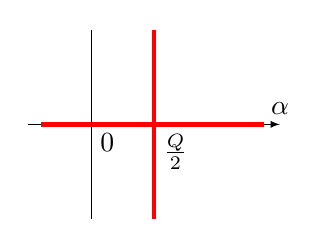
\begin{tikzpicture}[scale = .4, baseline=(current  bounding  box.center)]
  \draw[-latex, very thin] (-2, 0) -- (0, 0) node[below right] {$0$} -- (2, 0) node[below right] {$\frac{Q}{2}$} -- (4, 0)  -- (6, 0) node[above] {$\alpha$};
  \draw[red, ultra thick] (-1.6, 0) -- (5.5, 0);
  \draw[red, ultra thick] (2, -3) -- (2, 3);
  \draw[very thin] (0, -3) -- (0, 3);
 \end{tikzpicture}
\end{align}
We also need $\Delta$ to be bounded from below, and the natural bound is $\Delta(\alpha=\frac{Q}{2}) = \frac{Q^2}{4}=\frac{c-1}{24}$. This leads to $\alpha \in \frac{Q}{2}+i\mathbb{R}$, or rather $\alpha \in \frac{Q}{2}+i\mathbb{R}_+$ due to the reflection symmetry \eqref{eq:refm}. This is our guess for the spectrum for $c\in\mathbb{R}$, and we take it to hold for $c\in\mathbb{C}$ by analyticity.

Let us schematically write two- and three-point functions in Liouville theory, as well as OPEs:
\begin{align}
 \Big< V_{\alpha_1}V_{\alpha_2} \Big>  &=  B(\alpha_1)\delta(\alpha_1-\alpha_2)\ ,
 \label{eq:vv}
 \\
 \Big< V_{\alpha_1}V_{\alpha_2}V_{\alpha_3} \Big> & = C_{\alpha_1,\alpha_2,\alpha_3} \ ,
 \\
 V_{\alpha_1}V_{\alpha_2} &= \int_{\frac{Q}{2}+i\mathbb{R}_+} d\alpha \frac{C_{\alpha_1,\alpha_2,\alpha}}{B(\alpha)} \Big( V_\alpha + \cdots\Big)\ .
 \label{eq:v1v2}
\end{align}

In order to have reasonably simple crossing symmetry equations, we need degenerate fields. 
\begin{hyp}[Degenerate fields in Liouville theory]
 ~\label{hyp:degl}
 The degenerate fields $V_{\langle r, s\rangle}$, and their correlation functions, exist. 
\end{hyp}
Degenerate fields do not correspond to states in the spectrum, as the spectrum is made of Verma modules (not degenerate representations). 
On top of that, 
OPEs $V_{\langle r, s\rangle}V_\alpha$ then produce more fields outside the spectrum, for instance 
$V_{\langle 2, 1\rangle} V_\alpha \sim V_{\alpha-\frac{b}{2}} + V_{\alpha+\frac{b}{2}}$ with in general $\alpha\pm\frac{b}{2}\notin \frac{Q}{2}+i\mathbb{R}_+$. We assume that correlation functions involving $V_{\alpha\pm\frac{b}{2}}$ make sense by analytic continuation in $\alpha$. So, let us introduce notations for OPE coefficients of $V_{\langle 2, 1\rangle}$:
\begin{align}
 V_{\langle 2, 1\rangle} V_\alpha \sim C_+(\alpha) V_{\alpha-\frac{b}{2}} + C_-(\alpha)V_{\alpha +\frac{b}{2}}\ .
\end{align}


\section{Four-point functions}\label{sec:4pt}

Let us determine the three-point structure constant by solving crossing symmetry equations. We begin with the equations that come from four-point functions with degenerate fields. These equations are enough for uniquely determining the three-point structure constant.

\subsection{Single-valued four-point functions}

The four-point function $G(z) = \Big< V_{\langle 2, 1 \rangle}(z) V_{\Delta_1}(0)V_{\Delta_2}(\infty)V_{\Delta_3}(1) \Big>$ obeys second-order BPZ equations in $z$ and $\bar z$, and the most general solution is
\begin{align}
 G(z) = \sum_{i,j=\pm} c^{(s)}_{ij} \mathcal{F}^{(s)}_{\alpha_1-i\frac{b}{2}}(z) \mathcal{F}^{(s)}_{\alpha_1-j\frac{b}{2}}(\bar z)\ .
\end{align}
Conformal blocks behave as powers of $z$ near $z=0$ \eqref{eq:gsd}, and single-valuedness requires that we have the same power on the left and on the right. This implies $c^{(s)}_{+-} = c^{(s)}_{-+}=0$. By the same reasoning, single-valuedness near $z=1$ requires $c^{(t)}_{+-}=c^{(t)}_{-+}=0$. Now $c^{(t)}_{ij}$ and $c^{(s)}_{ij}$ are the coefficients of $G(z)$ in two different bases of solutions of the BPZ equation, and are related by a change of basis:
\begin{align}
 \mathcal{F}^{(s)}_{\alpha_1-i\frac{b}{2}}(z) = \sum_{j=\pm} F_{ij} \mathcal{F}^{(t)}_{\alpha_1-j\frac{b}{2}}(z) \quad \Rightarrow \quad \sum_{i,j=\pm} c^{(s)}_{ij} F_{ii'} F_{jj'} = c^{(t)}_{i'j'}\ .
\end{align}
In particular we have $0 = c^{(t)}_{+-}= c_{++}^{(s)} F_{++}F_{+-} + c_{--}^{(s)} F_{-+}F_{--}$, so that
\begin{align}
 \frac{c_{++}^{(s)}}{c_{--}^{(s)}} = -\frac{F_{-+}F_{--}}{F_{++}F_{+-}} 
 = \frac{\gamma(A)\gamma(B)\gamma(C-A)\gamma(C-B)}{\gamma(C)\gamma(C-1)}\quad \text{with} \quad \gamma(x) =\frac{\Gamma(x)}{\Gamma(1-x)}\ ,
 \label{eq:coc}
\end{align}
where the combinations $A,B,C$ of the momentums $\alpha_1,\alpha_2,\alpha_3$ are given in eq. \eqref{abc}.

This concludes the mathematical exercise of finding single-valued solutions of the hypergeometric equation. 
Now, in conformal field theory, the coefficients $c^{(s)}_{ij}$ are further constrained to be combinations of OPE coefficients and three-point structure constants, 
\begin{align}
 c_{++}^{(s)} = C_+(\alpha_1) C_{\alpha_1-\frac{b}{2},\alpha_2,\alpha_3} 
\quad , \quad 
c_{--}^{(s)}  = C_-(\alpha_1) C_{\alpha_1+\frac{b}{2},\alpha_2,\alpha_3}\ ,
\label{cs}
\end{align}
and eq. \eqref{eq:coc} becomes a shift equation for the dependence of $C_{\alpha_1,\alpha_2,\alpha_3}$ on $\alpha_1$,
\begin{align}
 \frac{C_+(\alpha_1) C_{\alpha_1-\frac{b}{2},\alpha_2,\alpha_3} }{C_-(\alpha_1) C_{\alpha_1+\frac{b}{2},\alpha_2,\alpha_3}} = \frac{\prod_{\pm,\pm} \gamma(\frac12 +b(\alpha_1-\frac{Q}{2}) \pm b(\alpha_2-\frac{Q}{2}) \pm b(\alpha_3-\frac{Q}{2}))}{\gamma(b(2\alpha_1-Q)) \gamma(1+b(2\alpha_1-Q))}\ .
 \label{eq:shift}
\end{align}
In order to find the three-point structure constant $C_{\alpha_1,\alpha_2,\alpha_3}$, we need to constrain the degenerate OPE coefficients $C_\pm(\alpha)$. To do this, we consider the special case where the last field is degenerate too, i.e. the four-point function $\Big\langle V_{\langle 2,1 \rangle}(z) V_\alpha(0) V_{\alpha}(\infty) V_{\langle 2,1 \rangle}(1)\Big\rangle$.
In this case, we have
\begin{align}
 c_{++}^{(s)} = C_+(\alpha)^2 B(\alpha-\tfrac{b}{2}) \quad , \quad c_{--}^{(s)} = C_-(\alpha)^2B(\alpha+\tfrac{b}{2}) \ ,
\end{align}
and eq. \eqref{eq:coc} boils down to 
\begin{align}
 \frac{C_+(\alpha)^2 B(\alpha-\tfrac{b}{2})}{C_-(\alpha)^2B(\alpha+\tfrac{b}{2})} 
 =  \frac{\gamma(-b(2\alpha-Q))}{\gamma(b(2\alpha-Q))} 
 \frac{\gamma(-b^2+b(2\alpha-Q))}{\gamma(-b^2-b(2\alpha-Q))} \ .
 \label{eq:shiftd}
\end{align}
Moreover, we could get the equations \eqref{eq:shift} and \eqref{eq:shiftd} with $b\to \frac{1}{b}$ by having $V_{\langle 1,2\rangle}$ instead of $V_{\langle 2,1\rangle}$ in our four-point functions. Next we will solve these equations. 


\subsection{Determining three-point structure constants}

In order to solve the shift equations for $C_{\alpha_1,\alpha_2,\alpha_3}$, we need a function that produces Gamma functions when its argument is shifted by $b$ or $\frac{1}{b}$. 

\begin{exo}[Upsilon function]
~\label{exo:upsilon}
 For $b>0$, show that there is a unique (up to a constant factor) holomorphic function $\Upsilon_b(x)$ that obeys the shift equations
 \begin{align}
  \frac{\Upsilon_b(x+b)}{\Upsilon_b(x)} = b^{1-2bx} \gamma(bx)\qquad \text{and} \qquad \frac{\Upsilon_b(x+\frac{1}{b})}{\Upsilon_b(x)} = b^{\frac{2x}{b}-1} \gamma(\tfrac{x}{b})\ .
\label{upup}
\end{align}
For $ib>0$, show that the meromorphic function 
\begin{align}
 \hat{\Upsilon}_b(x) = \frac{1}{\Upsilon_{ib}(-ix+ib)}\ ,
\end{align}
obeys shift equations that differ from eq. \eqref{upup} by $b^{\cdots} \to (ib)^{\cdots}$.
\end{exo}
The functions $\Upsilon_b(x)$ and $\hat\Upsilon_b(x)$ can respectively be defined for $\Re b>0$ and $\Re ib>0$ by analytic continuation. And we have 
\begin{align}
 \Upsilon_b(x) = \lambda_b^{(\frac{Q}{2}-x)^2}\prod_{m,n=0}^\infty f\left(\frac{\frac{Q}{2}-x}{\frac{Q}{2}+mb+nb^{-1}}\right) \quad \text{with} \quad f(x)=(1-x^2)e^{x^2}\ ,
\end{align}
where $\lambda_b$ is an unimportant $b$-dependent constant.
Using the functions $\Upsilon_b(x)$, let us write the ansatz
\begin{align}
 C_{\alpha_1,\alpha_2,\alpha_3} =  \frac{N_0 \prod_{i=1}^3 N(\alpha_i)}{\Upsilon_b(\alpha_1+\alpha_2+\alpha_3-Q) \Upsilon_b(\alpha_1+\alpha_2-\alpha_3)\Upsilon_b(\alpha_2+\alpha_3-\alpha_1)\Upsilon_b(\alpha_3+\alpha_1-\alpha_2)} \ ,
\end{align}
where $N_0$ is a function of $b$, and $N(\alpha)$ is a function of $b$ and $\alpha$. 
Then the shift equation \eqref{eq:shift} reduces to an equation that involves the dependence on $\alpha_1$ only, and that we write as
\begin{align}
 \frac{C_+(\alpha)N(\alpha-\frac{b}{2})}{C_-(\alpha)N(\alpha+\frac{b}{2})} = \frac{b^{4b(2\alpha-Q)}}{ \gamma(b(2\alpha-Q)) \gamma(1+b(2\alpha-Q))}\ .
\end{align}
Combining this equation with the shift equation \eqref{eq:shiftd}, we can eliminate the unknown degenerate OPE coefficients $C_\pm(\alpha)$, and we obtain
\begin{align}
 \frac{\left(N^2B^{-1}\right)(\alpha-\frac{b}{2})}{\left(N^2B^{-1}\right)(\alpha+\frac{b}{2})} = b^{8b(2\alpha-Q)} \frac{\gamma(-b(2\alpha-Q))}{\gamma(b(2\alpha-Q))} \frac{\gamma(-b^2-b(2\alpha-Q))}{\gamma(-b^2+b(2\alpha-Q))}\ .
\end{align}
Together with its image under $b\to b^{-1}$, this equation has the solution
\begin{align}
 \left(N^2B^{-1}\right)(\alpha) = \Upsilon_b(2\alpha)\Upsilon_b(2\alpha-Q)\ .
\end{align}
Therefore, we can only compute the combination $N^2B^{-1}$, and not the individual functions $B$ and $N$ that appear in the 
two- and three-point functions. This is because we still have the freedom of performing changes of field normalization $V_\alpha(z) \to \lambda(\alpha)V_\alpha(z)$. Under such changes, we have $B\to \lambda^2B$ and $N\to \lambda N$, while
the combination $N^2B^{-1}$ is invariant.

We now adopt the field normalization $N(\alpha)=\Upsilon_b(2\alpha)$, and we also choose $N_0=1$. 
% Field normalization such that C_+ = 1, and B(\alpha)B(Q-\alpha)=1.
We obtain the DOZZ formula (for Dorn, Otto, A.
Zamolodchikov and Al. Zamolodchikov),
\begin{align}
 C_{\alpha_1,\alpha_2,\alpha_3} =  \frac{\Upsilon_b(2\alpha_1) \Upsilon_b(2\alpha_2) \Upsilon_b(2\alpha_3)}{\Upsilon_b(\alpha_1+\alpha_2+\alpha_3-Q) \Upsilon_b(\alpha_1+\alpha_2-\alpha_3)\Upsilon_b(\alpha_2+\alpha_3-\alpha_1)\Upsilon_b(\alpha_3+\alpha_1-\alpha_2)} \ .
\label{caaa}
\end{align}
This formula holds if
$c\notin ]-\infty, 1]$ i.e. $b\notin i\mathbb{R}$. 
On the other hand, doing the replacements $\Upsilon_b\to \hat\Upsilon_b$ and $b^{\cdots} \to (ib)^{\cdots}$, we obtain a solution $\hat C$ that holds if  $c\notin [25,\infty[$ i.e. $b\notin \mathbb{R}$.

In the case of (generalized) minimal models, the momentums $\alpha_{\langle r,s\rangle}$ belong to a lattice with periods $b$ and $\frac{1}{b}$, so they are uniquely determined by the shift equations. The solution is given by $C$ or $\hat C$, which coincide. (Actually $C$ has poles when $\alpha_i$ take degenerate values, one should take the residues.)

In the case of Liouville theory, the solution is unique if $b$ and $b^{-1}$ are aligned, i.e. if $b^2\in\mathbb{R}$:
\begin{equation}
 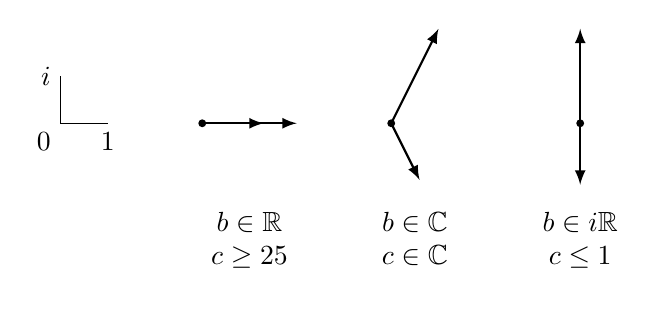
\begin{tikzpicture}[baseline=(current  bounding  box.center), scale = .6]
\draw (0, 2) node[left]{$i$} -- (0, 1) node[below left] {$0$} -- (1, 1) node[below] {$1$};
\draw [thick, latex-latex] (11,3) -- (11,1) node[fill, circle, minimum size = 1mm, inner sep = 0]{} -- (11,-.3);
\draw [thick, latex-latex] (8,3) -- (7,1) node[fill, circle, minimum size = 1mm, inner sep = 0]{}-- (7.6,-.2);
\draw [thick, latex-latex] (5,1) -- (3,1) node[fill, circle, minimum size = 1mm, inner sep = 0]{} -- (4.3,1) ;
\node at (4, -1.5){$\begin{array}{c} b\in \mathbb{R} \\ c\geq 25 \end{array}$};
\node at (7.5, -1.5){$\begin{array}{c} b\in \mathbb{C} \\ c\in\mathbb{C} \end{array}$};
\node at (11, -1.5){$\begin{array}{c} b\in i\mathbb{R} \\ c\leq 1 \end{array}$};
 \end{tikzpicture}
\end{equation}
However, for general values of $c$, both $C$ and $\hat C$ are solutions, and there are actually infinitely many other solutions. In order to prove the existence and uniqueness of Liouville theory, we have to determine which solutions lead to crossing-symmetric four-point functions.


\subsection{Crossing symmetry}

We have found that (generalized) minimal models are unique for all values of $c$, while Liouville theory is unique at least if $b^2\in\mathbb{R}$. We will now address the question of their existence. 

The $s$-channel decomposition of a Liouville four-point function reads 
\begin{align}
 \Big< V_{\alpha_1}(z) V_{\alpha_2}(0) V_{\alpha_3}(\infty) V_{\alpha_4}(1)\Big> = \int_{\frac{Q}{2}+i\mathbb{R}_+} d\alpha\ \frac{C_{\alpha_1,\alpha_2,\alpha} C_{\alpha,\alpha_3, \alpha_4}}{B(\alpha)} \mathcal{F}_{\alpha}^{(s)}(z) \mathcal{F}_{\alpha}^{(s)}(\bar z)\ ,
\end{align}
where the structure can be $C$ or $\hat C$. Let us accept that the conformal blocks $\mathcal{F}_{\alpha}^{(s)}(z)$ have poles when $\alpha = \alpha_{\langle r, s\rangle} $ \eqref{eq:ars}, the momentums for which the $s$-channel representation becomes reducible.
We now plot the positions of these poles (blue regions) relative to the integration line (red), depending on the central charge:
\begin{align}
 \newcommand{\polewedge}[3]{
\begin{scope}[#1]
\node[blue, draw,circle,inner sep=1pt,fill] at (0, 0) {};
\node[#3] at (0,0) {#2};
\filldraw[opacity = .1, blue] (0,0) -- (4, -4) -- (4, 4) -- cycle;
\end{scope}
}
\begin{array}{ccc}
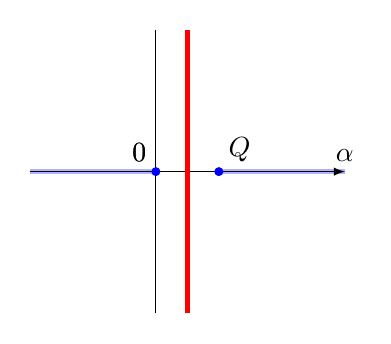
\begin{tikzpicture}[scale = .4, baseline=(current  bounding  box.center)]
 \draw[ultra thick, blue, opacity = .3] (0,0) -- (-4,0);
 \draw[ultra thick, blue, opacity = .3] (2,0) -- (6,0);
  \draw[-latex] (-4,0) -- (0, 0) node[above left] {$0$} -- (6,0) node [above] {$\alpha$};
  \draw (0, -4.5) -- (0, 4.5);
  \draw[ultra thick, red] (1, -4.5) -- (1, 4.5);
  \node[blue, draw,circle,inner sep=1pt,fill] at (0, 0) {};
\node[above left] at (0,0) {$0$};
\node[blue, draw,circle,inner sep=1pt,fill] at (2, 0) {};
\node[above right] at (2,0) {$Q$};
 \end{tikzpicture}
 & 
 \begin{tikzpicture}[scale = .4, baseline=(current  bounding  box.center)]
  \draw[-latex] (-4,0) -- (0, 0) node[above left] {$0$} -- (6,0) node [above] {$\alpha$};
  \draw (0, -4.5) -- (0, 4.5);
  \draw[ultra thick, red] (1, -4.5) -- (1, 4.5);
  \polewedge{rotate = 180}{$0$}{above left};
  \polewedge{shift = {(2, .3)}}{$Q$}{above right};
 \end{tikzpicture}
 &
 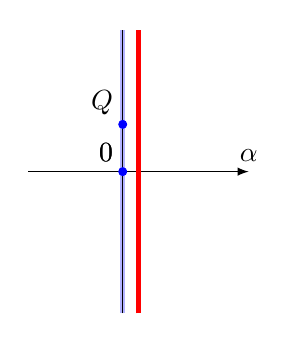
\begin{tikzpicture}[scale = .4, baseline=(current  bounding  box.center)]
  \draw[-latex] (-3,0) -- (0, 0) node[above left] {$0$} -- (4,0) node [above] {$\alpha$};
  \draw[ultra thick, blue, opacity = .3] (0, -4.5) -- (0, 4.5);
  \draw (0, -4.5) -- (0, 4.5);
  \draw[ultra thick, red] (.5, -4.5) -- (.5, 4.5);
  \node[blue, draw,circle,inner sep=1pt,fill] at (0, 0) {};
\node[above left] at (0,0) {$0$};
\node[blue, draw,circle,inner sep=1pt,fill] at (0, 1.5) {};
\node[above left] at (0,1.5) {$Q$};
 \end{tikzpicture}
 \vspace{3mm}
 \\
 c\in [25,\infty[ & c\notin ]-\infty, 1] \cup [25,\infty[ &  c\in ]-\infty, 1]
\end{array}
\end{align}
The four-point function built from $C$ is analytic on $c\notin ]-\infty,1]$. So if Liouville theory exists for $c\in [25,\infty[$, then it also exists for $c\notin ]-\infty,1]$, with the same structure constant $C$. 
On the other hand, the limit $c\to ]-\infty, 1]$ is singular. Actually, for $c\in ]-\infty, 1]$, the integration line has to be slightly shifted in order to avoid the poles. So the structure constant $\hat C$ is expected to be valid only for $c\in ]-\infty, 1]$.

That is how far we can easily get with analytic considerations. 
Let us now seek input from numerical tests of crossing symmetry. (See the associated \href{https://github.com/ribault/bootstrap-2d-Python/blob/master/Liouville_demo_2.ipynb}{Jupyter notebook}.)
We find that Liouville theory exists for all values of $c$, with the three-point structure constants $C$ for $c\notin ]-\infty,1]$, and $\hat C$ for $c\in ]-\infty, 1]$. 
We also find that generalized minimal models exist for all values of $c$, and minimal models exist at the discrete values of $c$ where they are defined. 
And we can numerically compute correlation functions with a good precision.

\section*{Acknowledgements}

I am grateful to the organizers of the Carg\`ese school, for challenging me to explain Liouville theory in about four hours.
I with to thank Bertrand Eynard, Riccardo Guida and Andr\'e Voros for helpful suggestions and comments.
And I am grateful to the participants of the Carg\`ese school, for their stimulating participation in the lectures.

\bibliographystyle{cft}
\bibliography{cft}

%\input{refs.tex}

\end{document}

